\chapter{Evaluierung der Programmiersprache Elm}
\label{sec:Evaluierung der Programmiersprache Elm}
\pagestyle{plain}

\section{Bewertungsmuster}
\label{sec:Bewertungsmuster}
Der folgende Teil dieser wissenschaftlichen Arbeit befasst sich mit der Entwicklung eines Modells, um die Programmiersprache Elm und ihre Nutzung als Frontend für Webapplikationen bewerten zu können. Dabei soll ein bereits fertiges Template von den ursprünglichen Programmiersprachen \ac{HTML}, \ac{CSS} und \ac{JS} in die Programmiersprache Elm portiert werden. Während der Entwicklung/Portierung wird die Programmiersprache Elm gegenüber mehreren Gesichtspunkten verglichen und ausgewertet.
Das fertige Template ist eine \ac{SPA} mit Elementen, wie sie typischerweise auf einer solchen Webseite vertreten sind. Eine \ac{SPA} ist, wie der Name bereits suggeriert, eine Webseite effektiv nur einer aktiven Seite und ohne Unterseiten (ausgenommen Impressum, AGB und Datenschutz). Die \ac{SPA} wird genutzt um ein Produkt oder Konzept schnell und einfach zu präsentieren, ohne den Nutzer mit Informationen zu überfluten und Unübersichtlichkeit in Form von tief verlinkten Unterseiten zu erzeugen. Oftmals wird eine SPA auch als Startseite benutzt und bietet nur eine geringe Anzahl an Funktionen.
Die fertige \ac{SPA} soll unter anderem die folgenden, typischen Elemente enthalten:
\begin{itemize}
\item Navigation mit Anchor-Elementen
\subitem{-} Verkleinern der Navigation nach $x$ Pixeln
\subitem{-} ScrollSpy zur Darstellung der aktuellen Position
\item Titelbild mit einem vertikal und horizontal zentriertem Text
\item Service-Sektion
\item Twitter-Bootstrap\ac{CSS} + Funktionen
\subitem{-} Vorgefertiges, responsive Design
\subitem{-} Hamburger Menü
\item Portfolio mit Bildern, wobei ein Klick einen asynchronen Request ausführt und Daten nach lädt
\item Formular zur Kontaktaufnahme mit Validierung der Korrektheit der eingegebenen Daten
\end{itemize}
Mit diesen Elementen kann eine typische SPA verwirklicht werden. Die Navigation bietet dabei die Möglichkeit für den Nutzer schnell zwischen einzelnen Sektionen der Seite zu wechseln. Das initiale Titelbild mit einem zentrierten Text gibt den Kontext der Präsentation an und soll das Interesse des Nutzers anregen. Die folgende Service-Sektion wird dazu genutzt, allgemeine Informationen über das beworbene Produkt anzuzeigen. In der darauf folgenden Portfolio-Sektion werden dem Nutzer mehrere Bilder des Produktes angezeigt, wobei ein Klick auf eines der Bilder dazu führt, dass ein Popup erzeugt wird in welches mit Hilfe eines AJAX-Requests Informationen asynchron vom Server angefordert und im Nachhinein geladen werden. Zuletzt kann sich der Nutzer für einen Newsletter anmelden. Die Eingaben des Nutzers sollen auf Richtigkeit überprüft werden.


\section{Bewertungskriterien}
\label{sec:Bewertungskriterien}
Während der Bearbeitung, respektive Überführung des Templates soll der erzeugte Code, sowie der Weg dahin analysiert werden. Hierbei sind Aspekte wie Wiederverwendbarkeit und Effizienz von großer Bedeutung. Aber auch die Produktivität während der Arbeit mit dem Code soll betrachtet werden. Die Bewertungskriterien setzen sich zum Großteil aus den zugrunde liegenden Kriterien aus dem Dokument XY der Washington University zusammen. Im Folgenden soll die Notwendigkeit der Kriterien und ihre eigentliche Bedeutung verständlich gemacht werden.
\iffalse
Dabei werden die Kriterien unterteilt in zwei Gruppen. Die erste Gruppe stellt externe Abhängigkeiten dar, also die Ansprüche eines Entwicklers an die Programmiersprache. Die zweite Gruppe zeigt interne Abhängigkeiten auf und setzt sich über die stark subjektiven Ansprüche und Einflüsse eines Entwicklers hinweg und versucht die Programmiersprache objektiv einzuordnen.

(http://www.cs.gordon.edu/courses/cs323/lectures-2009/LanguageEvaluationCriteria.pdf + http://courses.cs.washington.edu/courses/cse341/02sp/concepts/evaluating-languages.html)
\fi


\subsection{Entwicklungsgeschwindigkeit}
\label{sec:Entwicklungsgeschwindigkeit}
Gerade für Startups ist es wichtig, ein erstes Produkt so schnell wie möglich bereitzustellen. Die Entwickler müssen entsprechend mit wenigen Mitteln ein fertiges (Software-)Produkt ausliefern können, selbst wenn sie noch kein oder wenig Vorwissen zu einer Programmiersprache haben.
Dementsprechend sollte eine Programmiersprache nur eine geringe Anzahl an primitiven Konzepten aufweisen, die sich leicht erweitern lassen. Beispielsweise hat die Programmiersprache C standardmäßig keine Anreihung von Buchstaben, auch bekannt als $String$. Jedoch gibt es den Datentyp $char$, der einen einzelnen Buchstabe repräsentiert. Durch die Verknüpfung mehrerer $char$'s, kann letztendlich der Datentyp $String$ umgesetzt werden.


\subsection{Wartbarkeit}
\label{sec:Wartbarkeit}
Geschriebener Quellcode muss wartbar sein. Das bedeutet, dass Entwickler auch nach einem zeitlichen Abstand in der Entwicklung den Programmcode verstehen und entsprechend verändern kann. Dazu gehört, dass der Quellcode gut dokumentiert ist, respektive erläuternde Kommentare hinzugefügt wurden, oder der Code selbsterklärend ist. Auch sollten Funktionen sinnvoll und markant benannt werden, so dass dies bereits Aufschlüsse darüber gibt, was das Ziel der Methode ist. Ein weiterer Schritt um die Wartbarkeit von Quellcode zu gewährleisten sind Tests, durch die eine Methode und ihre eigentliche Funktion getestet und auf Fehler überprüft werden kann. Damit dieses Kriterium als erfüllt angesehen wird, muss der Quellcode mit Kommentaren in beliebiger Form versehen werden können. Besser wäre es, wenn eine Option zur automatischen Generierung von Informationen über beispielsweise den Aufbau einer Funktion oder des Moduls existiert.

\subsection{Zuverlässigkeit}
\label{sec:Zuverlässigkeit}
Für einen Entwickler von Software, egal wofür und mit welcher Programmiersprache gearbeitet wird, ist es wichtig, dass das ausgelieferte Programm letzten Endes fehlerfrei funktioniert. Dazu gehört, dass das Programm nicht unvorhergesehen abstürzt, andere Systeme beeinträchtigt oder dem späteren Nutzer der Software anderweitig Probleme beschert. In den meisten Fällen helfen die Editoren mit denen der Quellcode geschrieben wird bereits, indem syntaktische Fehler durch unterstreichen sichtbar, oder Vorschläge zur Vervollständigung des angefangenen Codes gemacht werden. Wichtig ist entsprechend, dass die Programmiersprache auf offensichtliche Fehler, entweder durch Plugins für den Editor oder durch den Compiler selbst, aufmerksam macht und sie somit verhindert und nicht erst im Produktionssystem den Fehler zulässt. Als Testfall wird Quellcode bewusst mit Fehlern versehen, die zu einem Absturz des Programmes während der Laufzeit führen würden. Erkennt der $elm-compiler$ diese Fehler oder umgeht den Absturz, gilt das Kriterium als erfüllt.


\subsection{Portabilität}
\label{sec:Portabilität}
Nicht alle Programmiersprachen und die damit erzeugten Programme funktionieren auf allen Endgeräten. Es kommt dabei sehr stark auf die Hardwarekomponenten und das Betriebssystem des Zielsystems an. Es ist wünschenswert, dass Quellcode nur einmal geschrieben und auf das Zielsystem übertragen werden kann, ohne großartige Änderungen am Quellcode vornehmen zu müssen. Letzten Endes wird versucht den Quellcode auf mehreren Zielsystemen zu kompilieren. Elm liefert Installationsanweisungen für die Betriebssysteme $Mac$, $Windows$ und allen Betriebssystemen, die $nodejs$ unterstützen. Gibt es keinerlei Differenz in Form von Fehlern oder Warnungen während des Kompilierens, gilt die Portabilität als erfüllt.


\subsection{Effizienz}
\label{sec:Effizienz}
„Zeit ist Geld.“ ist auch heute noch immer eine wahre Aussage. Entsprechend ist es von Vorteil, wenn Quellcode schnell erzeugt, getestet und als fertiges Produkt (Software) an den Kunden ausgeliefert werden kann. Dabei ist es wichtig, dass der Compiler den Quellcode schnell in ein lauffähiges Programm verwandelt und auch das daraus resultierende Programm effizient arbeitet, sprich schnell ist. Damit eine Aussage über die notwendige Zeit für das kompilieren des Quellcodes getroffen werden kann, wird der Code zehn mal kompiliert und die benötigte Zeit gemessen. Anschließend wird der höchste und niedrigste Wert verworfen. Im Anschluss wird das arithmetische Mittel der verbleibenden acht Werte ermittelt. TODO.
Die Performance der Programmiersprache wird nicht anhand des hier entwickelten Projektes, sondern der externen Applikation \cite{https://github.com/evancz/todomvc-perf-comparison/} TodoMVC Performance Comparison. Dieses Tool ermöglicht es, eine Beispiel-Applikation "TodoMVC", die in mehreren Programmiersprachen realisiert wurde, zu testen. Dabei werden automatisch gewisse Aktionen in der jeweiligen Sprache durchgeführt, die benötigte Zeit gemessen und am Ende gegenübergestellt. Mit Hilfe des Tools werden 20 Messungen durchgeführt und das Endergebnis betrachtet. Ist Elm signifikant schneller als die anderen getesteten Programmiersprachen, gilt das Kriterium als erfüllt. Die anderen Umgebungen der Applikation sind ebenso in nativem \ac{JS} oder einer zu \ac{JS} kompilierenden Programmiersprache geschrieben. Dadurch kann eine Aussage über die tatsächliche Effizienz der Applikation im Vergleich gemacht werden.



\subsection{Erlernbarkeit}
\label{sec:Erlernbarkeit}
Wie im vorherigen Punkt, ist es wirtschaftlich wichtig schnell zu arbeiten und Ergebnisse zu erbringen. Demzufolge sollte auch der Lernprozess schnell vonstatten gehen und die Programmiersprache eine gewisse Einfachheit in ihren Grundkonzepten verwirklichen, um dem Entwickler ein einfacheres Erlernen zu ermöglichen.



\subsection{Wiederverwendbarkeit}
\label{sec:Wiederverwendbarkeit}
Erzeugter Quellcode sollte nicht für jedes Projekt oder gar Modul innerhalb eines Projektes neu geschrieben und somit vervielfacht werden. Besser ist es wenn der Quellcode lediglich einmal geschrieben wird und von anderen Modulen benutzt werden kann. Dadurch vereinfacht sich auch die Wartbarkeit des Quellcodes, da Änderungen nur an einer Stelle vorgenommen werden müssen und sich so weniger Fehler einschleichen können.



\subsection{Lesbarkeit}
\label{sec:Lesbarkeit}
Quellcode muss lesbar sein. Gemeint ist damit, dass Befehle stets einen prägnanten, einfachen und möglichst kurzen Namen haben sollten. Des Weiteren ist es notwendig, dass der Sinn des geschriebenen Quellcodes beim ersten lesen verständlich wird. Jede Programmiersprache verfolgt dabei einen anderen Ansatz. Ist die Lesbarkeit gegeben, so kann Quellcode auch von Neulingen gelesen werden. Es ist für diese Neulinge nicht unbedingt notwendig die Syntax oder gar genaueres über einzelnen Befehle zu wissen, es reicht vollkommen aus, wenn das angestrebte Ziel des Quellcodes klar wird und adaptiert werden kann.



\subsection{Modularität}
\label{sec:Modularität_Analyse}
Mit der Zeit wächst ein Projekt. Zumeist steigt simultan auch die Zahl der Menschen, die an einem Projekt mitarbeiten, wodurch Quellcode sehr schnell unübersichtlich wird. Um Übersichtlichkeit zu gewährleisten wird der geschriebene Programmcode oftmals ausgelagert und in einzelne Module unterteilt, die wiederum logische Teilblöcke des gesamten Programmes darstellen. Die einzelnen Module sollten voneinander isoliert funktionieren, so dass Änderungen in Modulen nur eine Anpassung in der Kommunikation erfordern. Weiterhin kann durch Module der Zugriff auf bestimmte Funktionen gewährt oder verweigert werden.


\section{Ansprüche an eine Webapplikation}
\label{sec:ansprueche-webapp}
Diese Kriterien ermöglichen es, die Programmiersprache als solches anhand der eingebauten Möglichkeiten die diese bietet objektiv beurteilen zu können. Da sich diese wissenschaftliche Arbeit allerdings ausdrücklich mit der Evaluierung von Elm für Webapplikationen auseinandersetzt, müssen auch diese Kriterien untersucht werden und einen höheren Stellenwert bei der Bewertung einnehmen.
Webapplikationen können grundsätzlich in zwei Typen unterteilt werden. Zunächst gibt es die  \ac{SPA}, bestehend aus nur einer einzigen Seite, bei der typischerweise nur wenig  Programmlogik vorhanden ist und der Client lediglich die Informationen anzeigt. Des Weiteren gibt es die Rich-Internet-Applikationen\\
(RIA: http://www.itwissen.info/definition/lexikon/rich-Internet-application-RIA.html). Diese Art der Webapplikation besitzt im wesentlichen mehr Programmlogik, die der Client ausführen kann. Ein weiteres Merkmal sind oftmals auch die Anzahl der vorhandenen Unterseiten, wodurch wiederum mehr Logik erforderlich wird.
Bei der Erstellung einer \ac{SPA} muss generell weniger Aufwand betrieben werden, um eine fertige Präsentation zu erstellen.
Jede Webapplikation lebt von einem Frontend, sowie einem Backend. Typischerweise bezeichnet das Frontend dabei alle Komponenten, die an den Benutzeroberfläche des Nutzers gesendet werden. Dazu gehören unter anderem die Komponenten\ac{HTML},\ac{CSS} und\ac{JS}. Der Nutzer interagiert mit dieser Darstellung der Oberfläche.
Das Gegenstück zum Frontend stellt das sogenannte Backend dar. Dabei handelt es sich um Komponenten, die dem Webserver zugehörig sind. Unter anderem ist das zum Beispiel eine Datenbank, die eigentliche Webapplikation und natürlich der Webserver selbst. Der Nutzer agiert mit dem Backend nur über zuvor im Frontend eingerichtete Schnittstellen mit dem Backend.


\subsection{Browser Kompatibilität – Portabilität}
\label{sec:Browser Kompatibilität Portabilität}
Ein weiterer wichtiger Aspekt ist die Kompatibilität der Browser mit den genutzten Programmiersprachen. Da der Browser die Darstellung des\ac{HTML} und\ac{CSS} Quellcodes übernimmt, sowie die Manipulationen des DOM durch \ac{JS}, ist es wichtig, dass der Browser den vorhandenen Quellcode lesen und ausführen kann. Sämtliche Sprachen wie\ac{HTML},\ac{CSS} und \ac{JS} befinden sich im konstanten Wandel und werden stets weiter entwickelt.
Dabei werden nicht nur vorhandene Fehler behoben, sondern auch neue Eigenschaften hinzugefügt, sowie teilweise ersetzt oder verworfen. Diese Änderungen können darin münden, dass Nutzer unterschiedlicher Browser, auch unterschiedliche Ergebnisse angezeigt bekommen, manche Features gar nicht erst funktionieren oder die Applikation im schlimmsten Fall abstürzt. Natürlich muss die Applikation letzten Endes auch auf den gängigen Browsern fehlerfrei funktionieren, insbesondere die fünf meistgenutzten Browser Google Chrome, Safari, Internet Explorer, Firefox und Opera (vgl. Abbildung~\ref{fig:browser-may-2016}).
\iffalse
www.w3counter.com/trends\\+
https://www.w3counter.com/globalstats.php?year=2016&month=5
\fi

\begin{figure}[hb]
  \centering  
  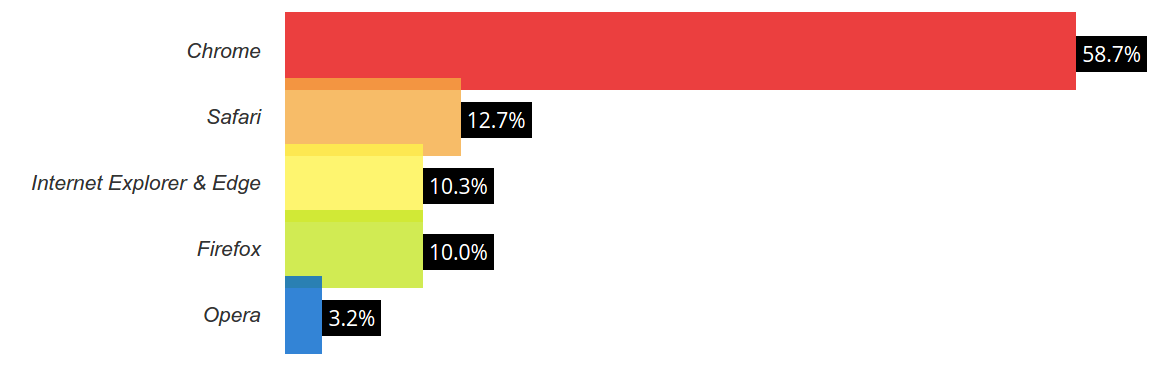
\includegraphics[scale=0.3]{img/browser_2016.png}
  \caption{Die fünf meistgenutzten Browser im Mai 2016}\label{fig:browser-may-2016}
\end{figure}

\subsection{Interoperabilität}
\label{sec:Interoperabilität_Analyse}
Auch bei den Webapplikationen ist es wichtig, bereits existente Frameworks und Problemlösungen nutzen zu können. Dementsprechend müssen externe\ac{JS} und\ac{CSS} Bibliotheken ohne große Probleme eingebettet werden können. Dies kann bequem über die vorhandenen\ac{HTML}-Tags und ihre Attribute gemacht werden.


\subsection{Asynchrones Laden}
\label{sec:Asynchrones Laden}
Nicht immer ist es sinnvoll, sämtliche Daten die auf einer Webseite angezeigt werden auch direkt an den Nutzer zu schicken. Sind beispielsweise große Datenmengen erst nach mehrmaligem Scrollen durch den Nutzer sichtbar, kann es ausreichen die Daten asynchron nachzuladen, sobald der Viewport, also der für den Nutzer sichtbare Bereich, sich diesem Inhalt nähert. Auf diese Weise kann der Server entlastet und die Ladezeit für den Nutzer verringert werden. Dieses Verhalten wird „Lazy Load“ genannt (XY). Besonders wenn davon auszugehen ist, dass der Nutzer nur einen sehr eingeschränkten Viewport oder eine schlechte Internetverbindung hat, bietet sich das asynchrone nachladen von Daten an.


\subsection{Dateigröße}
\label{sec:Dateigroesse}
Die Größe einer Datei wirkt sich auf die Dauer der Übertragungszeit aus. Ist die Datei groß, müssen entsprechend viele Informationen vom Server auf den Client des Nutzers übertragen werden, um die Webseite ansprechend darzustellen. Die Dateigröße kann mit einfachen Mitteln verringert werden. Beispielsweise können alle nicht unbedingt notwendigen Zeichen aus der Datei entfernt werden. Dazu gehören Zeichen wie „Leerzeichen“ (Whitespaces) oder Zeilenumbrüche. Doch auch die Verkürzung von Variablen ist denkbar. Anstelle von „EinZiemlichLangesWort“ reicht beispielsweise „a“ komplett aus. Offensichtlich muss die Variable im gesamten Code entsprechend umbenannt werden. Hierzu bedarf es Algorithmen, welche die Nutzung von Variablen genau untersuchen und Fehler durch Ersetzungen vermeiden.

\section{Empirische Analyse}
\label{sec:Empirische Analyse}
\subsection{Versuchsaufbau}
\label{sec:Versuchsaufbau}
Abbildung XY: Zeigt die Kommunikation zwischen Client und Webserver
Die Abbildung XY zeigt die geplante Kommunikation zwischen dem Client, also dem Nutzer und dem Webserver.
In Schritt 1 fordert der Nutzer die Webseite an, erzeugt also einen Request. Dieser geht in Schritt 2 bei dem Webserver ein und wird verarbeitet. Abhängig von der angeforderten URL erzeugt der Webserver dann eine Antwort, mit allen zu sendenden Informationen und dem dazugehörigen\ac{HTML},\ac{CSS} und\ac{JS} Code. Im nächsten Schritt 3 werden diese Daten zurück an den Client gesendet. Der Client nimmt die Daten entgegen, wie in Schritt 4 beschrieben. Des Weiteren macht der Client die Daten entsprechend sichtbar, so dass der Nutzer nun eine vollständige Präsentation der Webseite sieht. Schritt 5 beschreibt die mögliche Interaktion des Nutzers mit dem ihm präsentierten Dokument. Jede Interaktion führt zu einer Reaktion durch \ac{JS}, oder erzeugt einen neuen Request an den Server, womit wieder bei Schritt 1 begonnen wird. Das Einbinden von\ac{CSS} und\ac{JS} aus externen Quellen wird durch Schritt 6 verbildlicht.
Die gesamte Applikation wird von einem fertigen Template, programmiert in\ac{HTML},\ac{CSS} und\ac{JS} in die Programmiersprache Elm überführt, insofern möglich. Der daraus entstehende Elm-Quellcode wird daraufhin mit dem Elm-Compiler kompiliert zu \ac{JS}.
Um ein generelles Verständnis der Programmiersprache Elm zu bekommen, dient die Dokumentation auf http://elm-lang.org/docs als Hilfestellung. Dort besteht die Möglichkeit sich mit den grundlegenden Konzepten vertiefend auseinanderzusetzen und diese zu erlernen.
Die zugrunde liegende Elm-Version ist 0.17 und wird unter Ubuntu 14.04 64bit installiert. Als Editor wird Atom mit mehreren Elm-Plugins verwendet, so dass der geschriebene Code automatisch beim Speichern formatiert und durch den Compiler auf Fehler überprüft wird.
Lauffähig wird die geschrieben Applikation mit dem Elm-Compiler $elm-make$ gemacht und mit Google Chrome Version 50 getestet.
\subsection{Hypothesen und Vermutungen}
\label{sec:Hypothesen und Vermutungen}
Sämtliche Hypothesen wurden in der Tabelle~\ref{tab:Hypothesentabelle} zusammengefasst. Dabei beziehen sich die einzelnen Vermutungen jeweils auf eines der zuvor erläuterten Kriterien in den Kapiteln \nameref{sec:Bewertungskriterien} (\ref{sec:Bewertungskriterien}) und \nameref{sec:ansprueche-webapp} (\ref{sec:ansprueche-webapp}). Die Nummerierungen der Hypothesentabelle~\ref{tab:Hypothesentabelle} sind gleich der Auswertungstabelle~\ref{tab:Auswertungstabelle}, so dass ein Vergleich möglich ist.
\begin{table}[p]
\begin{tabular}{ | l | p{7.6cm} | }
	\hline
	\textbf{Kriterium} &\textbf{Hypothese}\\
	\hline
	1. Entwicklungsgeschwindigkeit & 1.1 Elm hat leicht erlernbare Grundkonzepte, die adaptiert und erweiterbar sind, um Produktivität für die Entwickler zu gewährleisten\\
	\hline
	2. Wartbarkeit & 2.1 Elm Code kann mindestens kommentiert werden, wenn nicht sogar eine Funktion zur automatischen Generierung von Signaturen einer Funktion existiert\\
	\hline
	3. Zuverlässigkeit & 3.1 Die Erweiterungen des Editors oder der Compiler warnt spätestens bei der Kompilierung, wenn nicht bereits während der Entwicklung vor syntaktischen Fehlern\\
	& 3.2  Gibt es keine Fehlermeldungen, wird die Applikation ohne Laufzeitfehler funktionieren\\
	& 3.3  Fehlermeldungen werden sehr spezifisch auf das eigentliche Problem hinweisen\\
	\hline
	4. Portabilität &  4.1 Die \ac{SPA} wird auf allen gängigen Browsern fehlerfrei dargestellt\\
	\hline
	5. Effizienz & 5.1 Der Kompiliervorgang wird nur wenige Sekunden dauern, jedoch mehr Zeit in Anspruch nehmen, als die herkömmliche Entwicklung mit reinem \ac{HTML}, \ac{CSS} und \ac{JS}\\
	&  5.2 Die erzeugte Elm-Applikation ist deutlich schneller während der Laufzeit\\
	\hline
	6. Wiederverwendbarkeit & 6.1 Codeteilen lassen sich problemlos auslagern und wiederverwenden\\
	\hline
	7. Modularität & 7.1 Ausgelagerte Codeteile sind isoliert voneinander und als einzelnes Modul nutzbar\\
	& 7.2 Module können Funktionen nach außen verbergen\\
	\hline
	8. Lesbarkeit &  8.1 Die automatische Formatierung des Elm-Codes macht diesen lesbarer und spart Zeit\\	
	\hline
	9. Dateigröße &  9.1 Die Dateigröße der Elm-Applikation wird kleiner als bei vergleichbaren Frameworks ausfallen\\
	\hline
	10. Interoperabilität &  10.1 Bestehende \ac{JS}-Skripte können mit der Elm-Applikation interagieren oder funktionieren bereits einwandfrei\\
	& 10.2 Bestehender \ac{CSS}-Code kann nativ in Elm eingebunden werden\\
	\hline
	11. Asynchrones Laden &  11.1 Elm erlaubt asynchrone Requests ohne Seiteneffekte zu erzeugen\\
	\hline
\end{tabular}
\caption{Aufstellung der Hypothesen}\label{tab:Hypothesentabelle}
\end{table}

\subsection{Versuchsdurchführung}
\label{sec:Versuchsdurchführung}
\subsubsection{Installation}
\label{sec:Installation}
Zunächst einmal ist es notwendig, Elm und die dazugehörigen Komponenten zu installieren. Im folgenden wird die Installation unter Ubuntu 14.04 64bit erklärt.
Elm wird über den NPM verbreitet. Um diesen zu installieren, sind folgende Kommandos auf der Kommandozeile auszuführen:

\begin{lstlisting}[language=bash]
$ sudo apt-get update
$ sudo apt-get install nodejs
$ sudo apt-get install npm
\end{lstlisting}

Dadurch wird das NodeJs-Paket installiert und ausführbar gemacht. Aufgrund der Tatsache, dass viele Pakete nicht $nodejs$, sondern $node$ als ausführbare Datei erwarten, wird noch sicherheitshalber ein Symlink erstellt.

\begin{lstlisting}[language=bash]
$ sudo ln -s /usr/bin/nodejs /usr/bin/node
\end{lstlisting}
Anschließend sollte überprüft werden, ob die Installation erfolgreich war und sowohl NodeJS, wie auch NPM verfügbar sind. Das Kommando \begin{lstlisting}[language=bash]
$ node -v && npm -v
\end{lstlisting}
liefert den Output, wie er in Abbildung XY zu sehen ist. Elm kann nun über die Paketverwaltung NPM mit dem Kommando 
$npm\,install\,-g\,elm$ installiert werden. Das $-g$ -Flag installiert die neueste Elm-Version global für alle Projekte auf dem System. Entfernt man es, wird die Zielversion nur für den aktuellen Ordner zugänglich gemacht. Um die hier behandelte Version 0.17 zu installieren, ist der Zusatz $@0.17$ direkt hinter dem globalen Flag notwendig.\\
Elm ist nun vollständig installiert und kann genutzt werden. Die Entwicklung in Atom wird unterstützt durch die Pakete $elm-format$\\ (https://github.com/triforkse/atom-elm-format), $language-elm$\\ (https://atom.io/packages/language-elm) und {$linter-elm-make$}\\ (https://atom.io/packages/linter-elm-make). Mit Hilfe dieser Pakete wird der Code automatisch beim speichern dem Style-Guide entsprechend formatiert, eventuelle Fehler bei der Kompilierung direkt im Editor sichtbar gemacht und der Code syntaktisch gefärbt, sowie Vorschläge zur Vervollständigung des geschriebenen Quellcodes gemacht. Da die Pakete ständig aktualisiert und verändert werden, wird an dieser Stelle von einer detaillierten Beschreibung zur Installation abgesehen und auf die Dokumentationen der einzelnen Pakete verwiesen (elm-lang.org).
Damit die geschriebene Applikation letztendlich im Browser aufrufen zu können, muss die Elm-Applikation zunächst in der\ac{HTML}-Datei aufgerufen und initialisiert werden. Dabei gibt es mehrere Möglichkeiten. Es ist sinnvoll hierbei zwischen vollautomatischem, sowie manuellem Grundaufbau zu unterschieden.
\subsubsection{Grundaufbau}
\label{sec:Grundaufbau}

1) Vollautomatisch – Elm-reactor\\
Mit Hilfe des $elm-reactor$, einem mitgelieferten Tools um den erzeugten Elm-Code lauffähig zu machen und die Applikation debuggen zu können, kann der gesamte Prozess der Kompilierung und Konfiguration eines Webservers automatisiert werden. Dafür muss lediglich der Ordner in dem die Elm-Applikation abgelegt wurde geöffnet und der $elm-reactor$ gestartet werden. 
Der Code kann automatisch kompiliert und zusätzlich eine $elm.html$ Datei erzeugt werden. Diese Datei wird dann mit dem gesamten kompilierten Elm-Code bestückt. Außerdem wird automatisch Code erzeugt, der den kompilierten\ac{JS}-Code ausführt. Für den Entwickler bedeutet dies, dass nur noch die erzeugten Dateien weitergegeben werden müssen. Die gesamte geschriebene Applikation ist darin enthalten und kann mit jedem Browser über die URL $http://localhost:8000/$ geöffnet werden, ohne die Notwendigkeit eines zusätzlichen Webservers. Die Abbildung ~\ref{fig:elm-reactor}) zeigt den laufenden Webserver.
\begin{figure}[hb]
\centering
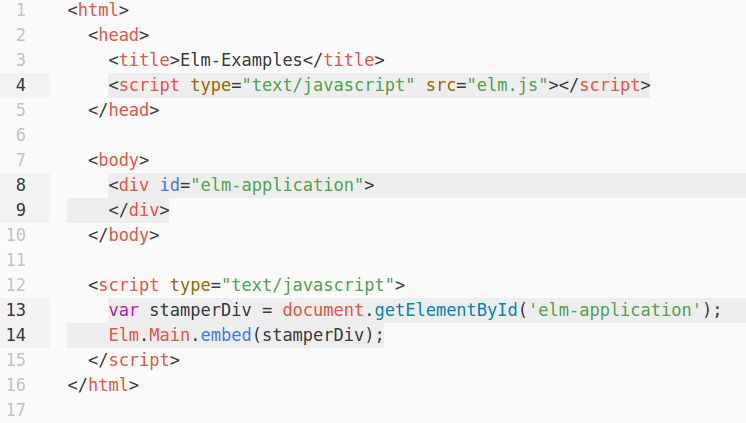
\includegraphics[scale=0.4]{img/elm-make_include_in_index.png}
\caption{Grundgerüst eines\ac{HTML}-Dokumentes, um die Elm Applikation zu laden}\label{fig:html-boilerplate}
\end{figure}
\begin{figure}[t]
\centering
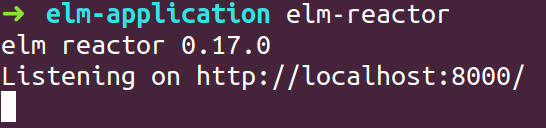
\includegraphics[scale=0.4]{img/elm-reactor.png}
\caption{Der gestartete Elm-Webserver}\label{fig:elm-reactor}
\end{figure}
Überlässt man dem Compiler das Einbinden der erzeugten\ac{JS}-Datei, so ist die gesamte Elm-Applikation im Vordergrund. Das ist nicht immer wünschenswert oder gar praktikabel. Einerseits, da externe Quellen für\ac{CSS} und\ac{JS} über natives Elm nicht reibungslos geladen werden können, andererseits weil nicht immer der gesamte darzustellende\ac{HTML}-Code nur in Elm geschrieben wurde. Dementsprechend gibt es auch die Möglichkeit, eine\ac{HTML}-Datei als Gerüst zu erzeugen, in die gezielt der\ac{JS}-Code der Elm-Applikation injiziert wird. Das Gerüst ist vollständig wie eine klassische\ac{HTML}-Datei aufgebaut. Abbildung~\ref{fig:html-boilerplate} zeigt das Grundgerüst des\ac{HTML}-Dokumentes. Codezeile $4$ bindet die kompilierte Elm-Datei. Der \ac{DOM}-Knoten in welchen die Applikation injiziert wird, ist in Zeile $8$ definiert. Das injizieren der Applikation geschieht in den Zeilen $13$ bis $14$ und erhält als Parameter den zuvor erwähnten \ac{DOM}-Knoten. Um die Elm-Applikation einfügen zu können, muss die Elm-Datei vorher in der Kommandozeile kompiliert werden mit dem Kommando \colorbox{lightgray}{\lstinline{elm-make Datei.elm --output=elm.js}}.
Bei dieser Art der Initialisierung kann nun noch zwischen drei weiteren Darstellungen unterschieden werden:
\begin{enumerate}
\item$fullscreen$: Der erzeugte Code der Applikation wird in den Body-Tag einer\ac{HTML}-Datei geladen und überschreibt den sonstigen\ac{HTML}-Code.

\item$embed$: Der erzeugte Code der Applikation wird in den übergebenen DOM-Knoten geladen.

\item$worker$: Initialisiert die Applikation ohne grafische Benutzeroberfläche.
\end{enumerate}
Der Vorteil bei Version 2, so wie es auch in der Abbildung~\ref{fig:html-boilerplate} realisiert wurde, ist, dass auch nur kleine Teile der gesamten Applikation in Elm implementiert werden können. Überlegt man ein bestehendes, möglicherweise komplexes Projekt zu portieren, genügt es kleinere Teile Stück für Stück zu portieren. Es muss nicht befürchtet werden, große Teile der bestehenden Applikation während der Portierung nutzlos zu machen. Ein weiterer Vorteil ist, dass externes\ac{CSS} und\ac{JS} in dem \ac{HTML}-Dokument über die \ac{HTML}-eigenen $<script>$-Tags geladen werden kann.
Zusätzlich zum Grundgerüst der $elm.html$ muss nun noch das Grundgerüst der eigentlichen Elm-App erstellt werden. Wie im Kapitel \nameref{sec:grundlagen} beschrieben, ist Elm nach einem \ac{MVU}-Konzept aufgebaut. Entsprechend sind das die unbedingt notwendigen Funktionen, die es zu realisieren gilt. Das standardmäßig mitgelieferte Paket $elm-lang/html$ liefert die sogenannten $Html.App$-Funktionen. Diese kümmern sich um die Bereitstellung und Auslieferung der Applikation, so dass sich Entwickler ganz auf die eigentliche Programmierung konzentrieren können. Dabei variieren stets die Übergabeparameter, wodurch die Applikation leicht erweitert und komplexer werden kann, ohne Neulinge direkt abzuschrecken. So verlangt die Funktion $Html.App.beginnerProgram$ nur die bekannten Funktionen $model$, $view$ und $update$. Hierbei können jedoch keine asynchronen Funktionen wie \ac{HTTP}-Requests genutzt werden.
Dafür gibt es die erweiterte Funktion $Html.App.program$, die als vierten Übergabeparameter sogenannte $subscriptions$ erwartet. $Subscriptions$ werden für die Kommunikation zwischen Elm und \ac{JS}, sowie die Verbindung zu Websockets genutzt.
Die dritte und letzte Möglichkeit ist die Funktion $Html.App.programWithFlags$. Hierbei wird die Übergabe eines initialen $Models$ an die Elm-Applikation ermöglicht, um den Zustand der Applikation dynamisch setzen zu können.
\begin{figure}[ht]
\centering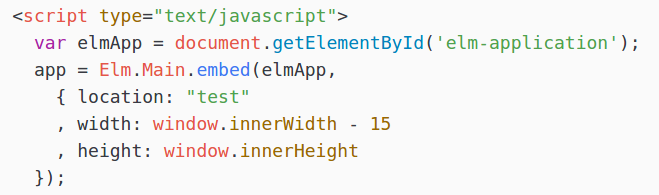
\includegraphics[scale=0.6]{img/programWithFlags_pass_data.png}
\caption{Eine beispielhafte Initialisierung der Elm-Applikation mit übergebenen Werten}\label{fig:programWithFlags}
\end{figure}
Abbildung~\ref{fig:programWithFlags} zeigt das Grundgerüst einer Elm-Applikation mit der Implementierung der Funktion $Html.App.programWithFlags$. Die $main$ Funktion erstellt dabei die eigentliche Applikation, während die Funktionen $model$, $view$ und $update$ jeweils den Zustand und die gewünschte Darstellung der Applikation beschreiben, sowie vorgeben, wie mit der Interaktion durch den Benutzer umgegangen wird. Die Funktion $subscription$ gibt in diesem Stand noch keinerlei Daten weiter und stellt eine Dummy-Funktion dar. $initialModel$ erzeugt beim Aufruf ein Model mit initialen Werten, die dem Model ($type\,alias\,Model$) entsprechen müssen. Durch das Grundgerüst der $elm.html$ und $Main.elm$-Datei kann die Applikation nun schrittweise erweitert und Funktionen hinzugefügt werden. Zuletzt wird der erzeugte Code modularisiert.

\subsubsection{Konstruktion des Views}
\label{sec:Konstruktion des Views}
TODO: Rewrite:
\begin{enumerate}
	\item Konstruktion des Views
	\subitem{-} Import der\ac{HTML}-Bibliothek
	\subitem{-} Aufruf der\ac{HTML}-Funktion
	\subitem{-} Signatur der\ac{HTML}-Funktion
	\subitem{-} Verschachtelung verschiedener Aufrufe
	\subitem{-} Unterschied\ac{HTML} vs. Elm
		\subsubitem{-}\ac{HTML}: Öffnende + schließende Tags (Fehleranfällig, unübersichtlich, schachtelbar in einer Zeile)
		\subsubitem{-} Elm: Einrückung (indention sensitive)
	\subitem{-} Mathematisch ausdrücken, dass Elm-Code im Gegensatz zu\ac{HTML} 'kürzer' ist
	\subitem{-} Fehleranfälligkeit von\ac{HTML} klarstellen
\end{enumerate}


Lorem ipsum dolor sit amet, consetetur sadipscing elitr, sed diam nonumy eirmod tempor invidunt ut labore et dolore magna aliquyam erat, sed diam voluptua. At vero eos et accusam et justo duo dolores et ea rebum. Stet clita kasd gubergren, no sea takimata sanctus est Lorem ipsum dolor sit amet. Lorem ipsum dolor sit amet, consetetur sadipscing elitr, sed diam nonumy eirmod tempor invidunt ut labore et dolore magna aliquyam erat, sed diam voluptua. At vero eos et accusam et justo duo dolores et ea rebum. Stet clita kasd gubergren, no sea takimata sanctus est Lorem ipsum dolor sit amet. Lorem ipsum dolor sit amet, consetetur sadipscing elitr, sed diam nonumy eirmod tempor invidunt ut labore et dolore magna aliquyam erat, sed diam voluptua. At vero eos et accusam et justo duo dolores et ea rebum. Stet clita kasd gubergren, no sea takimata sanctus est Lorem ipsum dolor sit amet.   

Duis autem vel eum iriure dolor in hendrerit in vulputate velit esse molestie consequat, vel illum dolore eu feugiat nulla facilisis at vero eros et accumsan et iusto odio dignissim qui blandit praesent luptatum zzril delenit augue duis dolore te feugait nulla facilisi. Lorem ipsum dolor sit amet, consectetuer adipiscing elit, sed diam nonummy nibh euismod tincidunt ut laoreet dolore magna aliquam erat volutpat.   

Ut wisi enim ad minim veniam, quis nostrud exerci tation ullamcorper suscipit lobortis nisl ut aliquip ex ea commodo consequat. Duis autem vel eum iriure dolor in hendrerit in vulputate velit esse molestie consequat, vel illum dolore eu feugiat nulla facilisis at vero eros et accumsan et iusto odio dignissim qui blandit praesent luptatum zzril delenit augue duis dolore te feugait nulla facilisi.   

Nam liber tempor cum soluta nobis eleifend option congue nihil imperdiet doming id quod mazim placerat facer possim assum. Lorem ipsum dolor sit amet, consectetuer adipiscing elit, sed diam nonummy nibh euismod tincidunt ut laoreet dolore magna aliquam erat volutpat. Ut wisi enim ad minim veniam, quis nostrud exerci tation ullamcorper suscipit lobortis nisl ut aliquip ex ea commodo consequat.   

Duis autem vel eum iriure dolor in hendrerit in vulputate velit esse molestie consequat, vel illum dolore eu feugiat nulla facilisis.   

At vero eos et accusam et justo duo dolores et ea rebum. Stet clita kasd gubergren, no sea takimata sanctus est Lorem ipsum dolor sit amet. Lorem ipsum dolor sit amet, consetetur sadipscing elitr, sed diam nonumy eirmod tempor invidunt ut labore et dolore magna aliquyam erat, sed diam voluptua. At vero eos et accusam et justo duo dolores et ea rebum. Stet clita kasd gubergren, no sea takimata sanctus est Lorem ipsum dolor sit amet. Lorem ipsum dolor sit amet, consetetur sadipscing elitr, At accusam aliquyam diam diam dolore dolores duo eirmod eos erat, et nonumy sed tempor et et invidunt justo labore Stet clita ea et gubergren, kasd magna no rebum. sanctus sea sed takimata ut vero voluptua. est Lorem ipsum dolor sit amet. Lorem ipsum dolor sit amet, consetetur sadipscing elitr, sed diam nonumy eirmod tempor invidunt ut labore et dolore magna aliquyam erat.   

Consetetur sadipscing elitr, sed diam nonumy eirmod tempor invidunt ut labore et dolore magna aliquyam erat, sed diam voluptua. At vero eos et accusam et justo duo dolores et ea rebum. Stet clita kasd gubergren, no sea takimata sanctus est Lorem ipsum dolor sit amet. Lorem ipsum dolor sit amet, consetetur sadipscing elitr, sed diam nonumy eirmod tempor invidunt ut labore et dolore magna aliquyam erat, sed diam voluptua. At vero eos et accusam et justo duo dolores et ea rebum. Stet clita kasd gubergren, no sea takimata sanctus est Lorem ipsum dolor sit amet. Lorem ipsum dolor sit amet, consetetur sadipscing elitr, sed diam nonumy eirmod tempor invidunt ut labore et dolore magna aliquyam erat, sed diam voluptua. At vero eos et accusam et justo duo dolores et ea rebum. Stet clita kasd gubergren, no sea takimata sanctus.   

\iffalse
Das erste sichtbare Modul der fertigen SPA ist die Navigationsleiste. Sie soll dem Nutzer die Möglichkeit bieten schnell und einfach einen Überblick über die vorhandenen Themen auf der Webseite zu erhalten und direkt mit einem Klick auf den Reiter zu einem Thema zu springen. Damit die Navigation während des gesamten Besuches möglich ist, soll die Navigationsleiste `fixed` sein, also am oberen Bildschirmrand fest verankert bleiben und mit scrollen.
Jedes Modul der dargestellten Seite besteht aus\ac{HTML}-Code. Folglich müssen\ac{HTML}-Tags mit Elm generiert werden. Seit dem neuesten Release von Elm (Version 0.17) wurden einige Pakete die sich für die Webentwicklung nutzen lassen zusammengeführt in das Paket `elm-lang/html`. Es erlaubt die Erzeugung von\ac{HTML} und\ac{CSS} mit nativem Elm-Code. In Elm können\ac{HTML}-Tags mit bereitgestellten Funktionen aus diesem Paket erzeugt werden. Ein\ac{HTML} `div`-Tag wird mit der gleichnamigen Funktion `div` erzeugt. Die Funktion erwartet zusätzlich zwei Argumente. Einerseits eine Liste von\ac{HTML}-Attributen wie `class`, `id` oder `href`, andererseits eine Liste von weiteren\ac{HTML}-Tags, insofern Code geschachtelt wird. Die Signatur für diese Funktion lautet wie folgt:
`div (List Html.Attribute msg) (List Html.Html msg)`
Entsprechend dieser Signatur wird in Abbildung XY gezeigt, wie die `div`-Funktion in Elm nach der Kompilierung in\ac{HTML} dargestellt wird.
Nicht nur die Erstellung eines\ac{HTML}-Tags, sondern auch die Zuweisung von Attributen ist in Elm eine Funktion. So sieht man in Abbildung XY ebenso, wie eine Klasse (`class`) und ID einem Element hinzugefügt wird. Da in Elm sämtliche Funktionen „pure functions“, also reine Funktionen sind, hat der Entwickler die Sicherheit, dass das Resultat der Funktion immer gleich bleibt.
Des Weiteren ist es möglich die\ac{HTML}-Elemente nativ in Elm mit\ac{CSS}-Styling zu versehen. Dafür wird die gleichnamige Funktion `style` aus dem Paket genutzt. Auch diese Funktion erwartet eine Liste von Argumenten, jeweils mit einem Schlüssel (hier:\ac{CSS}-Eigenschaft) und dem dazugehörigen Wert. Zur Zeit ist es nicht problemlos möchlich nativ in Elm eine externe\ac{CSS}-Datei zu integrieren. Corey Trampe (https://gist.github.com/coreytrampe/a120fac4959db7852c0f) hat eine Möglichkeit gefunden, jedoch wird bei dieser Lösung die Seite zunächst ohne jegliches Styling dargestellt, während ein asynchroner Request die externe\ac{CSS}-Datei lädt. Sobald dieser Vorgang abgeschlossen ist, wird das heruntergeladene Styling angewandt. Der zeitliche Abstand zwischen initialem Laden und der Anwendung des Styles hat ein sichtbares „flackern“ zur Folge, wodurch eine Nutzung in einem fertigen System entfällt. Alternativ werden alle zu ladenden\ac{CSS}-Dateien im\ac{HTML}-Grundgerüst über den\ac{HTML}-Tag `link` eingebunden.
\fi

\subsubsection{Überführung des Views}
\label{sec:Überführung des Views}
Für die Darstellung einer SPA wird ein fertiges und kostenloses Theme von `startbootstrap.com` verwendet. Im Zuge dessen werden alle verfügbaren Dateien heruntergeladen und die zuvor erstellten Dateien `elm.html` und `Main.elm` in denselben Ordner verschoben.
Das Grundgerüst der `elm.html` muss nun in die `index.html` überführt werden, so dass die Elm-Applikation weiterhin in den vorhandenen\ac{HTML}-Code injiziert wird.
Zunächst einmal muss der\ac{HTML}-Code des Themes in ausführbaren Elm-Code umgeschrieben werden, damit Elm Zugriff auf den kompletten `view` bekommt. Nur so kann Elm die Interaktion des Benutzers mit den\ac{HTML}-Elementen abfangen und entsprechend darauf reagieren. Um nicht den kompletten\ac{HTML}-Code der `index.html` per Hand in Elm-Code überführen zu müssen, wird das Tool `html-to-elm` genutzt (http://mbylstra.github.io/html-to-elm/). Dieses Online-Tool erlaubt es\ac{HTML}5-konformen Code in lauffähigen Elm-Code zu überführen. Der erzeugte Elm-Code wird dann in der `Main.elm`-Datei von der `view`-Funktion zurückgegeben., muss also entsprechend dort eingefügt werden.
Um Modularität zu gewährleisten, wird jede Sektion der SPA, wie zum Beispiel die Navigation, die Team-Sektion oder der Footer im ersten Schritt in eine eigene Funktion ausgelagert. Jede dieser Funktionen wird dann in der `view`-Funktion aufgerufen und ergibt am Ende die gesamte Webseite. Auf diese Weise können die einzelnen Teile der SPA unabhängig voneinander modifiziert und auf Korrektheit überprüft werden. Im nächsten Schritt wird der gesamte View-Code modularisiert.

\subsubsection{Modularisierung}
\label{sec:Modularisierung}
Damit ein Entwickler den Überblick über den vorhandenen Quellcode behält ist es sinnvoll einzelne Teile der Applikation in mehrere Dateien und Ordner zu verschieben. Eine solche Strukturierung hilft dabei die womöglich fehlerbehafteten Teile der Applikation zu finden und beispielsweise die Programmlogik noch deutlicher von der Applikationsdarstellung zu trennen. Dabei werden die einzelnen Funktionen des Views, also die für die Darstellung verantwortlichen Programmteile, ausgelagert in eigene Module. Dasselbe wird für die `Update` und `Model` relevanten Funktionen durchgeführt. Die notwendigen Funktionen eines jeden Moduls werden dann im Gegenzug vom Hauptmodul importiert und an den entsprechenden Stellen aufgerufen.\\\\
\noindent\textbf{View}\\
Jede bisherige Funktion aus dem View wird in den Ordner `View` verschoben und als gleichnamiges Modul benannt. Jedes Modul bekommt dabei den Namen des Ordners in dem es zu finden ist, gefolgt vom Namen des Views, dass es darstellt. Das für die Navigation verantwortliche Modul wird  entsprechend mit `module View.Navigation exposing (view)` initialisiert und gibt die Funktion `view` an jedes importierende Modul frei.
Dieser Schritt dient lediglich der besseren Strukturierung des Quellcodes und der Vereinfachung für den Entwickler. Abbildung XY zeigt die Haupt-`view`-Funktion nachdem sämtliche Teile des `View`s modularisiert und entsprechend importiert wurden.\\\\
\noindent\textbf{Update}\\
Auch die Programmlogik kann modularisiert werden und wird dafür in den Unterordner $Update$ verschoben. Hierfür werden sämtliche Typdeklarationen ($Msg$), sowie die dazugehörige Funktion $update$ in das neue Modul `Update.Update` verschoben und auch die notwendigen Pakete hinzugefügt. Von außen kann auf das $Update$-Modul, nachdem es importiert wurde, mit dem Namespace $Update$ zugegriffen werden.\\\\
\textbf{Model}\\
Letztlich wird noch das $model$, das sämtliche Daten die den Status der Applikation beschreiben enthält, in ein eigenes Modul im Unterordner $Model$ überführt. Die Einbindung dieses Moduls funktioniert analog zur Modularisierung von $Update$ und $View$.
Mit Hilfe dieser Modularisierung wird das angestrebte \ac{MVU}-Konzept von Elm besonders deutlich.

\subsubsection{Asynchrones Laden}
\label{sec:Asynchrones Laden - Analyse}
Das fertige Template bietet die Möglichkeit auf einen Portfoliobeitrag zu klicken. Durch diesen Klick wird ein Modal geöffnet, in das weitere Informationen dargestellt werden. Üblicherweise werden diese zusätzlichen Informationen in einer \ac{SPA} nachgeladen, um das initiale Laden der Applikation zu verkürzen und nur wirklich notwendige Daten anzuzeigen. Die bestehende Elm-Applikation wird nun um das Feature des asynchronen Ladens von Informationen erweitert.
Zunächst muss das $model$ erweitert und angepasst werden, da dies die einzige Möglichkeit in einer Elm-Applikation ist, Daten beziehungweise den Status der Applikation zu speichern. Das `model` bekommt entsprechend ein weiteres Feld `async-content : String`.
Bei einem Klick auf eines der Portfoliobeiträge soll entsprechend das Modal geöffnet und ein Titel präsentiert werden. In diesem Beispiel wird über eine externe API ein zufälliger String angefordert, vom Server generiert und dann an die Elm-Applikation zurückgegeben. Ebenso wäre es möglich einen Server für das Backend zu erstellen, auf dem eine Datenbank läuft, so dass Daten asynchron angefordert werden können. In diesem Fall ist es jedoch nicht notwendig ein zusätzliches Backend zu konfigurieren.
Ein solcher asynchroner Request stellt im Grunde eine Verletzung des Konzeptes von Elm dar, dass es keinerlei Seiteneffekte gibt. Da nicht bekannt ist, wann der Request endet und welchen Status die Antwort besitzt (Failed, Success, ..?), ist zunächst nicht vorhersehbar, wie der Status der Applikation nach dem Request aussehen wird. Um dieses Problem zu vermeiden, ist es notwendig alle möglichen Fälle , also den Fall einer erfolgreichen, sowie fehlerhaften Übertragung, zu behandeln. Auf diese Weise ist gewährleistet, dass die Applikation sich nicht plötzlich in einem nicht definierten Zustand befindet.
Einen asynchronen Request in Elm auszuführen bedarf mindestens zweier zusätzlicher Funktionen und der Importierung der Bibliotheken $Http$, $Json.Decode$ und $Task$. Des Weiteren muss der Klick auf das Portfolio-Element abgefangen werden. Dafür gibt es die $onClick$ Funktion aus der $Html.Events$-Bibliothek. Sie bekommt die auszuführende Funktion als Parameter, sieht also wie folgt aus: `onClick Update.GetRandomString`. Die möglichen `Types` von eingehenden Nachrichten (`Msg`/Klicks) wird erweitert um `GetRandomString`, sowie auch die `update`-Funktion um diesen Typ erweitert werden muss. Der entsprechende `update`-Fall `GetRandomString` gibt dann das `model`, sowie einen Effekt `fetchAsync` zurück. Die Definition dieses Effektes ist der Grund, weshalb hier von einem `managed Effect` die Rede ist und der Seiteneffekt kontrolliert verläuft. `fetchAsync` ist hierbei erneut eine Funktion, die eine Nachricht (`Msg`) an die `update`-Funktion mit dem Ergebnis des Requests zurückgibt . Elm führt den Request in Form eines `Task` aus und erwartet eine Funktion für den Fall einer erfolgreichen Übertragung, sowie eine Funktion für jeglichen Fehlerfall. In beiden Fällen wird die entsprechende Funktion ausgeführt und an die `update`-Funktion zurückgegeben. Hier wird, insofern notwendig, ein neues `model` mit veränderten Werten erzeugt und letztlich das Ergebnis auf dem Bildschirm des Nutzers sichtbar gemacht.\\
TODO: Allgemeiner beschreiben. Bei Bezug auf den Anwendungsfall, Abbildung einfügen.

\subsection{Beobachtungen}
\label{sec:Beobachtungen}
Während der Entwicklung der Elm-Applikation kam es zu unvorhergesehenen Problemen, sowie teilweisen Erkenntnissen. Diese Beobachtungen werden im folgenden stichpunktartig zusammengefasst und anschließend erläutert.
\begin{enumerate}[label*=\arabic*.]

\item Externes \ac{CSS} kann nicht nativ über Elm geladen werden
	\begin{enumerate}[label*=\arabic*.]
		\item Inline-\ac{CSS} muss manuell mehrfach abgeändert werden
		\item Keine Schachtelung möglich
		\item Browser kann inline-\ac{CSS} nicht zwischenspeichern
	\end{enumerate}
\item Ein\ac{HTML}-Element benötigt in Elm weniger Zeichen
	\begin{enumerate}[label*=\arabic*.]
		\item \ac{HTML}-Code benötigt in Elm keine schließenden Klammern. Anders als \ac{HTML} arbeitet Elm mit Einrückungen. Die gleichnamigen Funktionen um ein \ac{HTML}-Element zu erzeugen benötigen dementsprechend lediglich den Funktionsaufruf, gefolgt von den zwei Argumenten. Das bedeutet, dass nativer Code in Elm kürzer und weniger anfällig für Flüchtigkeitsfehler wie beispielsweise das Schließen eines Tags ist. Der Entwickler wird weniger syntaktische Fehler machen.
	\end{enumerate}
\item Vertikale und horizontale Zentrierung eines Elementes ist umfangreicher als vorerst erwartet
	\begin{enumerate}[label*=\arabic*.]
		\item Obwohl Elm ein Paket für genau dieses Anwendungsgebiet besitzt, ist die Anwendung dennoch weder simpel, noch voll funktionsfähig. Es bedarf einiger Transformationen der Elemente, um sie in nutzbare, validen \ac{HTML}-Code zu formatieren. Zuletzt trifft der Entwickler auf die Problematik, zusätzlich noch die explizite Größe des Fensters mit einbeziehen zu wollen, so dass das Element den gesamten Bildschirm ausfüllt und einen zentrierten Text beinhaltet. Die Fenstergröße zu ermitteln stellt ein größeres Hindernis dar, als zunächst erwartet. Die Möglichkeiten sind hier, halbwegs dynamisch die Fenstergröße bei der Initiierung der Elm-Applikation an diese weiter zureichen, oder über Ports abzufangen, wenn sich die Fenstergröße geändert hat. Die erste Lösung hilft nur, wenn die Größe des Fensters nicht weiter verändert wird. Dies kann jedoch nicht gewährleistet werden, wodurch die Lösung entfällt. Die zweite Lösung hingegen erzeugt eine zusätzliche Abhängigkeit zwischen Elm und externem \ac{JS}. Zuletzt bleibt noch die altbekannte Möglichkeit mittels \ac{CSS} den Text in einem Element beidseitig zu zentrieren. Hierfür kann das externe \ac{CSS}-Framework Flexbox zuhilfe gezogen werden. Flexbox kümmert sich um die horizontale und vertikale Platzierung von Elementen, ohne auf die \ac{CSS}-Eigenschaft „float“ zurückgreifen zu müssen, die gerade bei tief verschachtelten Elementen Probleme verursacht.
		
		\item Das Paket `elm-lang/window` stellt eine Funktion `resize` zur Verfügung, die bei jeder Veränderung der Fensterdimensionen über eine sogenannte `subscription` in Elm einen Aufruf der `update` Funktion auslöst, an jene die neuen Fensterdimensionen (X, Y) weitergereicht werden.
	\end{enumerate}

\item Elm-Compiler
	\begin{enumerate}[label*=\arabic*.]
		\item Kompiliert abhängig von der Tiefe der Elemente
		\begin{enumerate}[label*=\arabic*.]
			\item Entwickler muss lesbaren Code erzeugen, da Elm sensitiv auf Tabs reagiert (vs\ac{HTML}: $<div><span></span></div>$ wo unendliches verschachteln auch in einer Zeile möglich ist)
		\end{enumerate}
	\end{enumerate}

\item TODO:
	\begin{enumerate}[label*=\arabic*.]
		\item Fehlende Beispiele importieren
		\item Umschreiben der Beispiele
	\end{enumerate}
\end{enumerate}



\subsection{Auswertung}
\label{sec:Auswertung}
\begin{table}[h]
\centering
\begin{tabular}{ | l | c | }
	\hline
	\textbf{Kriterium} & \textbf{Erfüllt}\\
	\hline
	1. Entwicklungsgeschwindigkeit & \\
	1.1 & \checkmark\\
	\hline
	2. Wartbarkeit & \\
	2.1  & \checkmark\\
	\hline
	3. Zuverlässigkeit & \\
	3.1  & \checkmark\\
	3.2  & \checkmark\\
	3.3  & \checkmark\\
	\hline
	4. Portabilität & \\
	4.1  & ausstehend\\
	\hline
	5. Effizienz & \\
	5.1  & \checkmark\\
	5.2  & ausstehend\\
	\hline
	6. Wiederverwendbarkeit & \\
	6.1  & \checkmark\\
	\hline
	7. Modularität & \\
	7.1  & \checkmark\\
	7.2  & \checkmark\\
	\hline
	8. Lesbarkeit & \\
	8.1  & \checkmark\\	
	\hline
	9. Dateigröße & \\
	9.1  & ausstehend\\
	\hline
	10. Interoperabilität & \\
	10.1  & \checkmark\\
	10.2  & Nein/Nur bedingt\\
	\hline
	11. Asynchrones Laden & \\
	11.1  & \checkmark\\
	\hline
\end{tabular}
\caption{Auswertung der Versuchskriterien}
\label{tab:Auswertungstabelle}
\end{table}
TODO: Importieren der schriftlichen Auswertung der Tabelle~\ref{tab:Auswertungstabelle}

 1.1. Elm hat leicht erlernbare Grundkonzepte, die adaptiert und erweiterbar sind, um Produktivität für die Entwickler zu gewährleisten.
 
 2.1. Elm Code kann mindestens kommentiert werden, wenn nicht sogar eine Funktion zur automatischen Generierung von Signaturen einer Funktion existiert
 --> Kommentare können mit `--` (single-line) oder `{- a comment - }` erstellt werden. Eine vollautomatische, explizite Erstellung der Signaturen besteht derzeit nicht. Der Compiler wird jedoch nach dem Kompiliervorgang einen Signaturvorschlag geben. Dieser Vorschlag ist auf einer niedrigeren Ebene, als es eine Deklaration wäre, ist jedoch ausreichend und wesentlich sinnvoller als eine Signatur komplett unberücksichtigt zu lassen. Beispiel: Abbildung XY ($compiler_sig_suggestion$ + $compiler_own_sig$)
 ```
 type alias Model = { counter: Int }
 increaseModel: Model -> Model
 increaseModel model =
     {model | counter = model.counter + 1}
 
 vs. Kompiliervorschlag
 type alias Model = { counter: Int }
 increaseModel: { a | counter : number } -> { a | counter : number }
 increaseModel model =
     {model | counter = model.counter + 1}
 ```
 
 3.1. Die Erweiterungen des Editors oder der Compiler warnt spätestens bei der Kompilierung, wenn nicht bereits während der Entwicklung vor syntaktischen Fehlern
 --> Syntaktische Fehler werden vom Compiler erkannt und ein Fehler angezeigt. Der Fehler wird unterstützt durch einen Hinweis auf die mögliche Fehlerquelle (Abbildung XY – $Compiler_syntax_error$). Die Fehlermeldung wird erst nach der Kompilierung eingeblendet.
 ```
 div [ id "elm-view" ]
         [ Navigation.view model
             Header.view
         , Services.view]
 ```
 
 3.2. Gibt es keine Fehlermeldungen, wird die Applikation ohne Laufzeitfehler funktionieren
 --> Aufgrund der Garantien, dass es keine Seiteneffekte gibt und alle Variablen unveränderlich sind, ist die Korrektheit syntaktische und semantische Korrektheit des Codes gewährleistet. Lediglich die logische Implementierung eines Algorithmus kann noch Fehler aufweisen, dies kann jedoch nicht von einem Compiler überprüft werden.
 3.3. Fehlermeldungen werden sehr spezifisch auf das eigentliche Problem hinweisen
 --> Wie in Abbildung iii.i zu sehen ist, gibt der Compiler nicht nur an, in welcher Zeile ein Fehler gefunden wurde, sondern liefert zusätzlich noch einen Hinweis, worin eine wahrscheinliche Fehlerquelle liegt. In diesem Beispiel weißt der Compiler auf das fehlende Komma als Fehlerquelle hin.
 
 4.1  1. Die SPA wird auf allen gängigen Browsern fehlerfrei dargestellt
 --> AUSSTEHEND
 
 5.1. Der Kompiliervorgang wird nur wenige Sekunden dauern, jedoch mehr Zeit in Anspruch nehmen, als die herkömmliche Entwicklung mit reinem\ac{HTML},\ac{CSS} und\ac{JS}
 --> Bei der herkömmlichen Entwicklung ist kein expliziter Kompiliervorgang notwendig, stattdessen übernimmt der Browser die Darstellung des übergebenen\ac{HTML},\ac{CSS} und\ac{JS} Quellcodes. Der Kompiliervorgang der Elm-Applikation dauert wie in Abbildung XY  zu sehen ist im Durchschnitt XY Sekunden. Es wurde 10x gemessen, der höchste und niedrigste Wert gestrichen und dann das arithmetische Mittel der verbleibenden 8 Messungen ermittelt.
 
 5.2  2. Die erzeugte Elm-Applikation ist deutlich schneller während der Laufzeit
 --> AUSSTEHEND (Abbildung - Performance - Evtl. neu?)
 
 6. 1. Codeteilen lassen sich problemlos auslagern und wiederverwenden
 --> Der komplette View wurde von einer großen Darstellung in mehrere Funktionen unterteilt und letztlich in ein eigenes Modul überführt. Analog dazu wurden auch das Model, sowie die Update-Funktion ausgelagert. Das einmalig definierte `Model` kann in sämtlichen Modulen wiederverwendet werden, auch die einzelnen Funktionen eines jeden Moduls finden erneut Verwendung, insofern gewünscht.
 
 7.1. Ausgelagerte Codeteile sind isoliert voneinander und als einzelnes Modul nutzbar
 --> Diese Eigenschaft ist gegeben.
 7.2. Module können Funktionen nach außen verbergen
 --> Jedes Modul kann mit dem Stichwort `expose` einzelne Funktionen nach außen hin zugänglich machen. Das importierende Modul wiederum kann einzelne Funktionen in den derzeitigen globalen `Scope` laden.
 
 8.1. Die automatische Formatierung des Elm-Codes macht diesen lesbarer und spart Zeit
 --> Fehler werden Dank der Formatierung schnell sichtbar.
 
 9.1. Die Dateigröße der Elm-Applikation wird kleiner als bei vergleichbaren Frameworks ausfallen
 --> Die kompilierte Elm-Applikation hat eine Größe von etwa 300kb. Allerdings kann diese Größe um etwa 60Prozent verringert werden, wenn der Code `minified` wird.
  
  10.1. Bestehende\ac{JS}-Skripte können mit der Elm-Applikation interagieren oder funktionieren bereits einwandfrei
  --> Die Integration vorhandener\ac{JS}-Skripte verlief problemlos. Benötigt ein externes Skript Daten von der Elm-Applikation, so kann mit Hilfe von `Ports` eine gesicherte Kommunikation in beide Richtungen stattfinden.
  
  10.2. Bestehender\ac{CSS}-Code kann nativ in Elm eingebunden werden
  --> Das Einbinden von\ac{CSS} Quellen ist derzeit nicht ohne Probleme nativ in Elm möglich. Es verursacht ein „flackern“ und ist nicht für den Gebrauch in einem fertigen System geeignet.\ac{CSS}-Klassen und `inline-styling` sind jedoch nativ in Elm implementiert und erlauben ein Styling der Elemente. Externes\ac{CSS} muss jedoch über das Grundgerüst der\ac{HTML}-Datei eingebunden werden.
  
  11.1. Elm erlaubt asynchrone Requests ohne Seiteneffekte zu erzeugen
  --> Ein asynchroner Request stellt implizit einen Seiteneffekt dar, wird in Elm allerdings als gemanagter Seiteneffekt bezeichnet. In jedem Fall ist der Nutzer gezwungen eine Funktion bei einer fehlerhaften Übertragung zu übergeben, die dann die erwartenden Typen/Werte liefert.
  
  
  
  
  1. Installation sehr einfach
  1. externe Abhängigkeiten werden automatisch installiert
  2. Installation war schnell
  3. Erklärung zur Installation war deutlich
  2. Modularität möglich
  1. Jedes View-Element als eigenes Modul
  1. Paralleles arbeiten möglich
  2. Entwickler bekommen nur die notwendigen Informationen für das Interface
  3. Tools
  1.\ac{HTML}2ELM sehr hilfreich
  1. Kleinere Fehler
  1. ' verursacht Fehler (Weiterfolgende Divs wurden vernachlässigt)
  2. required --> required '' (wants Bool, got String); novalidate same
  2. Elm-Compiler
  1. Fehler von\ac{HTML}2ELM (2. Punkt) wurden sofort erkannt
  2. Fehlende Funktionen für\ac{HTML} und\ac{CSS} Attribute wurden in den Fehlermeldungen vorgeschlagen („Did you mean Html.Attributes.required?“ für „required true“)
  4. Erklärungen der Elm-Struktur in den Guides sehr gut